%% fcup-thesis.tex -- document template for PhD theses at FCUP
%%
%% Copyright (c) 2015 João Faria <joao.faria@astro.up.pt>
%%
%% This work may be distributed and/or modified under the conditions of
%% the LaTeX Project Public License, either version 1.3c of this license
%% or (at your option) any later version.
%% The latest version of this license is in
%%     http://www.latex-project.org/lppl.txt
%% and version 1.3c or later is part of all distributions of LaTeX
%% version 2005/12/01 or later.
%%
%% This work has the LPPL maintenance status "maintained".
%%
%% The Current Maintainer of this work is
%% João Faria <joao.faria@astro.up.pt>.
%%
%% This work consists of the files listed in the accompanying README.

%% SUMMARY OF FEATURES:
%%
%% All environments, commands, and options provided by the `ut-thesis'
%% class will be described below, at the point where they should appear
%% in the document.  See the file `ut-thesis.cls' for more details.
%%
%% To explicitly set the pagestyle of any blank page inserted with
%% \cleardoublepage, use one of \clearemptydoublepage,
%% \clearplaindoublepage, \clearthesisdoublepage, or
%% \clearstandarddoublepage (to use the style currently in effect).
%%
%% For single-spaced quotes or quotations, use the `longquote' and
%% `longquotation' environments.


%%%%%%%%%%%%         PREAMBLE         %%%%%%%%%%%%

%%  - Default settings format a final copy (single-sided, normal
%%    margins, one-and-a-half-spaced with single-spaced notes).
%%  - For a rough copy (double-sided, normal margins, double-spaced,
%%    with the word "DRAFT" printed at each corner of every page), use
%%    the `draft' option.
%%  - The default global line spacing can be changed with one of the
%%    options `singlespaced', `onehalfspaced', or `doublespaced'.
%%  - Footnotes and marginal notes are all single-spaced by default, but
%%    can be made to have the same spacing as the rest of the document
%%    by using the option `standardspacednotes'.
%%  - The size of the margins can be changed with one of the options:
%%     . `narrowmargins' (1 1/4" left, 3/4" others),
%%     . `normalmargins' (1 1/4" left, 1" others),
%%     . `widemargins' (1 1/4" all),
%%     . `extrawidemargins' (1 1/2" all).
%%  - The pagestyle of "cleared" pages (empty pages inserted in
%%    two-sided documents to put the next page on the right-hand side)
%%    can be set with one of the options `cleardoublepagestyleempty',
%%    `cleardoublepagestyleplain', or `cleardoublepagestylestandard'.
%%  - Any other standard option for the `report' document arclass can be
%%    used to override the default or draft settings (such as `10pt',
%%    `11pt', `12pt'), and standard LaTeX packages can be used to
%%    further customize the layout and/or formatting of the document.

%% *** Add any desired options. ***
%PDF
%\documentclass[a4paper,narrowmargins,11pt,oneside,draft,onehalfspaced,singlespacednotes]{fcup-thesis}
%\documentclass[a4paper,narrowmargins,11pt,oneside,onehalfspaced,singlespacednotes]{fcup-thesis}
%Print
%\documentclass[draft,a4paper,narrowmargins,11pt,twoside,openright,onehalfspaced,singlespacednotes]{fcup-thesis}
\documentclass[a4paper,narrowmargins,11pt,twoside,openright,onehalfspaced,singlespacednotes]{fcup-thesis}

%% *** Add \usepackage declarations here. ***
%% The standard packages `geometry' and `setspace' are already loaded by
%% `ut-thesis' -- see their documentation for details of the features
%% they provide.  In particular, you may use the \geometry command here
%% to adjust the margins if none of the ut-thesis options are suitable
%% (see the `geometry' package for details).  You may also use the
%% \setstretch command to set the line spacing to a value other than
%% single, one-and-a-half, or double spaced (see the `setspace' package
%% for details).
% Overfull statements
\pretolerance=150
\setlength{\emergencystretch}{3em}
% Overfull end
\usepackage[english]{babel}
\usepackage{helvet} %To replace arial fonts
\usepackage{lipsum}
\usepackage[utf8]{inputenc}


%%% Additional useful packages
%%% ----------------------------------------------------------------
\usepackage{array}
\usepackage{amsmath}  
\usepackage{amssymb}
\usepackage{amsfonts}
\DeclareFontFamily{OT1}{pzc}{}
\DeclareFontShape{OT1}{pzc}{m}{it}{<-> s * [0.900] pzcmi7t}{}
\DeclareMathAlphabet{\mathpzc}{OT1}{pzc}{m}{it}
%Titles need to be 14 pt => Large in \normaltext 11pt
\usepackage{titlesec}
\titleformat*{\section}{\Large\bfseries}
\titleformat*{\subsection}{\Large\bfseries}
\titleformat*{\subsubsection}{\Large\bfseries}
%Titles need to be 14 pt => Large in \normaltext 11pt
\usepackage{amsthm}      
\usepackage[ruled,algochapter]{algorithm2e}
\usepackage{algorithmic}
\usepackage{bm}
\usepackage[mathscr]{euscript}
\usepackage{graphicx}       
\usepackage{psfrag}         
\usepackage{fancyvrb}    
\usepackage{float}
\usepackage{ltablex}
\usepackage[square,sort,comma,numbers]{natbib}        
\usepackage{bbding}         
\usepackage{dcolumn}        
\usepackage{booktabs} 
\usepackage{multirow}
\usepackage{paralist}     
\usepackage{ifdraft}  
\usepackage{indentfirst}    
\usepackage[nottoc,notlof,notlot]{tocbibind}
\usepackage{url}
\usepackage{tabularx}
%use font size for captions like 8pt -> normalisize 11pt, scriptsize->8pt
\usepackage[font={scriptsize}]{caption}
\usepackage[font={scriptsize}]{subcaption}
\captionsetup{font=scriptsize}

\usepackage[unicode]{hyperref}
\usepackage{xcolor}


\hypersetup{pdftitle=Obstacle avoidance framework based on reach sets, 
            pdfauthor=Alojz Gomola,
            colorlinks=false,
            urlcolor=blue,
            pdfstartview=FitH,
            pdfpagemode=UseOutlines,
            pdfnewwindow,
            breaklinks
          }
\usepackage{array}
\newcolumntype{L}[1]{>{\raggedright\let\newline\\\arraybackslash\hspace{0pt}}m{#1}}
\newcolumntype{C}[1]{>{\centering\let\newline\\\arraybackslash\hspace{0pt}}m{#1}}
\newcolumntype{R}[1]{>{\raggedleft\let\newline\\\arraybackslash\hspace{0pt}}m{#1}}         
\newcolumntype{B}{X}
\newcolumntype{S}[1]{>{\hsize=#1\textwidth}X}

\newcommand{\FIGDIR}{./Pics}    %%% directory containing figures
\newcommand{\twolinecellr}[2][r]{%
  \begin{tabular}[#1]{@{}r@{}}#2\end{tabular}}
\newcommand{\secState}[1]{
	\ifdraft{(#1) }{}
}
\theoremstyle{plain}
\newtheorem{theorem}{Theorem}
\newtheorem{lemma}[theorem]{Lemma}
\newtheorem{proposition}[theorem]{Proposition}

\theoremstyle{plain}
\newtheorem{definition}{Definition}
\newtheorem{problem}{Problem}
\newtheorem{example}{Example}
\newtheorem{assumption}{Assumption}

\theoremstyle{remark}
\newtheorem*{corollary}{Corollary}
\newtheorem*{note}{Note}




\newenvironment{dokaz}{
  \par\medskip\noindent
  \textit{Proof}.
}{
\newline
\rightline{\SquareCastShadowBottomRight}
}

\newenvironment{constraints}[1]{
  \par\medskip\noindent
  \textit{Constraints #1} \\
}{
\newline
\rightline{\SquareCastShadowBottomRight}
}


%\bibliographystyle{plainnat}     %% Author (year) style
\bibliographystyle{unsrt}        %% [number] style
\setcitestyle{square}

% Section  3.7 Challenge list
\newif\ifproblemchallenge   %# Build block for problem challenges
\problemchallengetrue       %# Show comments

\newcommand{\R}{\mathbb{R}}
\newcommand{\N}{\mathbb{N}}

\DeclareMathOperator{\pr}{\textsf{P}}
\DeclareMathOperator{\E}{\textsf{E}\,}
\DeclareMathOperator{\var}{\textrm{var}}
\DeclareMathOperator{\sd}{\textrm{sd}}


\newcommand{\T}[1]{#1^\top}        

\newcommand{\goto}{\rightarrow}
\newcommand{\gotop}{\stackrel{P}{\longrightarrow}}
\newcommand{\maon}[1]{o(n^{#1})}
\newcommand{\abs}[1]{\left|{#1}\right|}
\newcommand{\dint}{\int_0^\tau\!\!\int_0^\tau}
\newcommand{\isqr}[1]{\frac{1}{\sqrt{#1}}}
\newcommand{\norm}[1]{\left\lVert#1\right\rVert}


\newcommand{\pulrad}[1]{\raisebox{1.5ex}[0pt]{#1}}
\newcommand{\mc}[1]{\multicolumn{1}{c}{#1}}
\newcommand{\TBD}[1]{\color{red}\emph{--TBD:}#1\color{black}}

%%%%%%%%%%%%%%%%%%%%%%%%%%%%%%%%%%%%%%%%%%%%%%%%%%%%%%%%%%%%%%%%%%%%%%%%
%%                                                                    %%
%%                   ***   I M P O R T A N T   ***                    %%
%%                                                                    %%
%%  Fill in the following fields with the required information:       %%
%%   - \degree{...}       name of the degree obtained                 %%
%%   - \department{...}   name of the graduate department             %%
%%   - \gradyear{...}     year of graduation                          %%
%%   - \author{...}       name of the author                          %%
%%   - \title{...}        title of the thesis                         %%
%%%%%%%%%%%%%%%%%%%%%%%%%%%%%%%%%%%%%%%%%%%%%%%%%%%%%%%%%%%%%%%%%%%%%%%%

%% *** Change this example to appropriate values. ***
\degree{Doctor of Philosophy}
\department{Departamento de Matem\'{a}tica}
\gradyear{2019}
\author{Alojz Gomola}
\title{Obstacle Avoidance Framework based on Reach Sets}

%% *** NOTE ***
%% Put here all other formatting commands that belong in the preamble.
%% In particular, you should put all of your \newcommand's,
%% \newenvironment's, \newtheorem's, etc. (in other words, all the
%% global definitions that you will need throughout your thesis) in a
%% separate file and use "\input{filename}" to input it here.


%% *** Adjust the following settings as desired. ***

%% List only down to subsections in the table of contents;
%% 0=chapter, 1=section, 2=subsection, 3=subsubsection, etc.
\setcounter{tocdepth}{3}

%% Make each page fill up the entire page.
\flushbottom


%%%%%%%%%%%%      MAIN  DOCUMENT      %%%%%%%%%%%%

\begin{document}

%09-Apendixes
	\appendix
	\setcounter{chapter}{5}
	% Confict resolution schemes
	\cleardoublepage

\chapter[Conflict Resolution]{Conflict Resolution}

   
		\subsection{(R) Cooperative Conflict Resolution}\label{sec:cooperativeConflictResolution}


\paragraph{Idea:} There is a \emph{final decision maker} (absolute authority) in conflict resolution. This authority is \emph{UTM} or \emph{air traffic attendant} with higher priority. The future \emph{UTM system} is such authority. The approach to mixed conflict resolution is mentioned in \cite{ramasamy2014towards}, based on navigation \cite{ramasamy2013novel}. This is similar to our approach. 

\begin{note}
    \emph{Open Issue:} Decentralized model with UTM as approver of directives is possible, but that is topic for own research.
\end{note}

\paragraph{Goal:} UAS is obligated to follow up committed mission plan with given precision.  There is one to five percent  allowed deviations for ATM mission plans.     Similar rates are achievable according to \cite{ramasamy2014towards}.  This requirement is given by \cite{icao4444} ICAO 4444 document for ATM operations.

\begin{figure}[H]
    \centering
    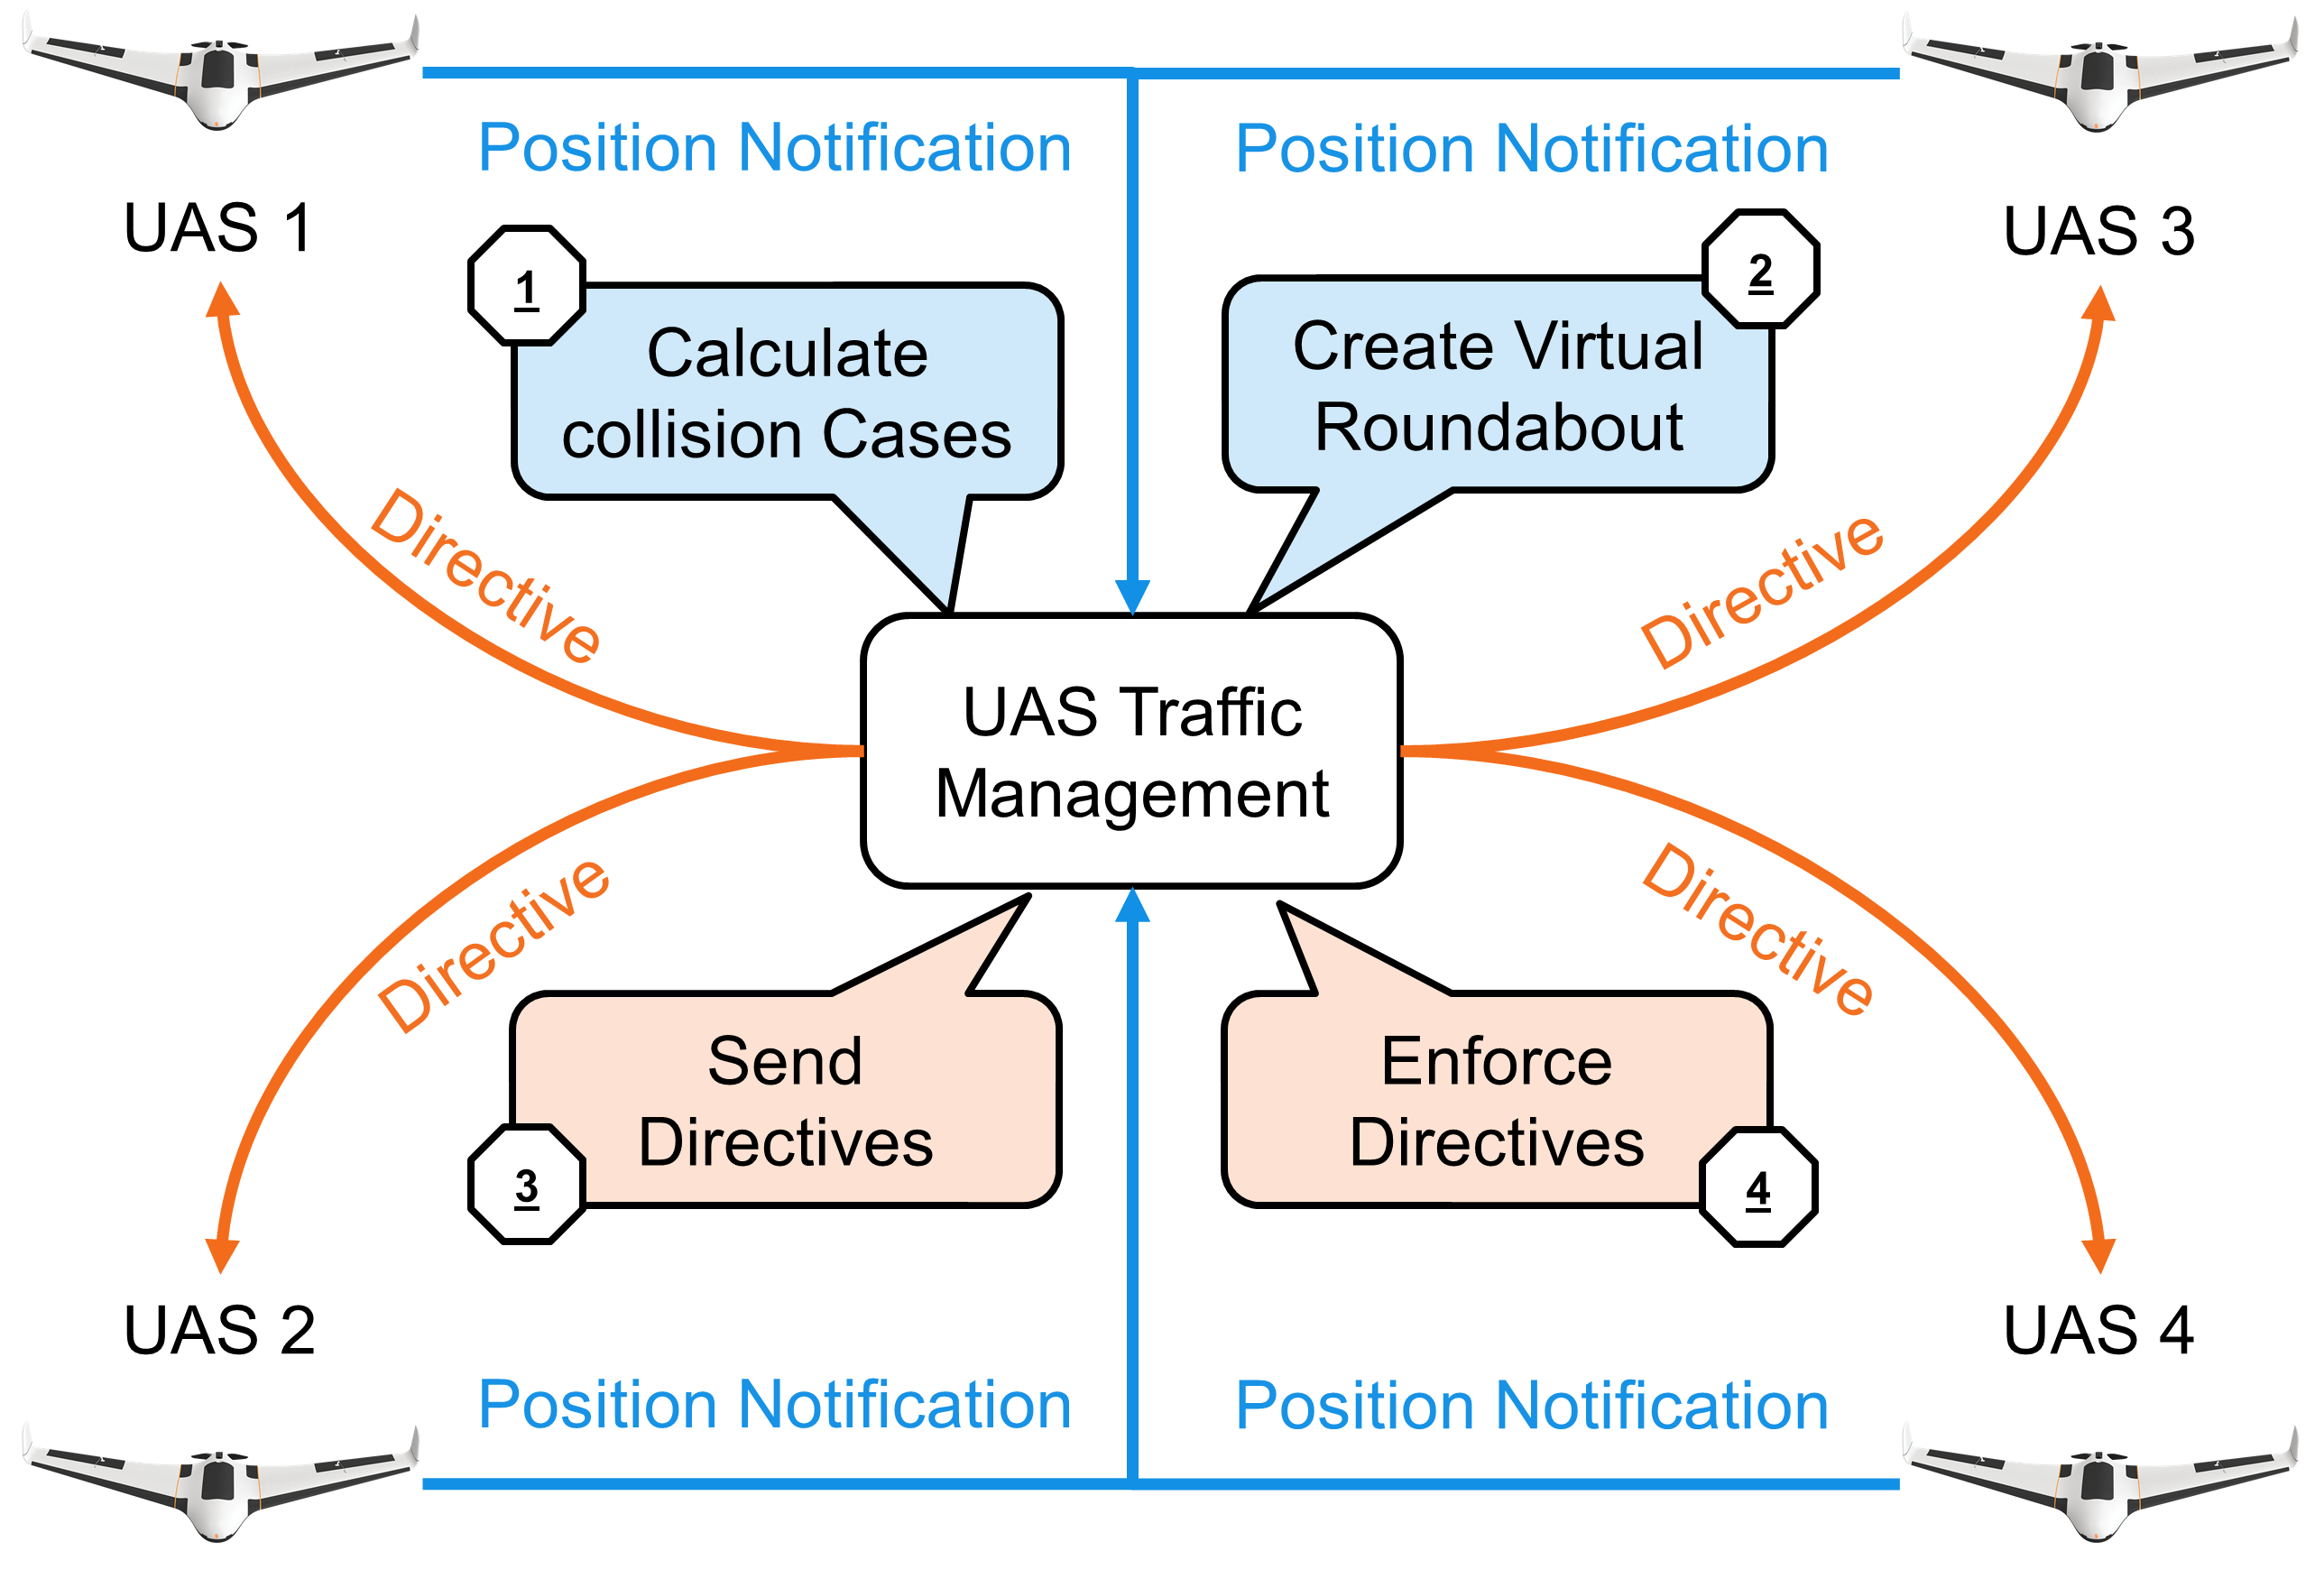
\includegraphics[width=0.7\linewidth]{\FIGDIR/RE003CooperativeResolution} 
    \caption{Cooperative conflict resolution via UTM authority.}
    \label{fig:CooperativeConflictResolutionUTM}
\end{figure}

\paragraph{Cooperative conflict resolution} (fig. \ref{fig:CooperativeConflictResolutionUTM}) shows functional diagram of one \emph{UTM time-frame} there  are following actors:
\begin{enumerate}
    \item \emph{Unmanned Autonomous System} (UAS) equipped with necessary navigation and communication modules, providing the unique \emph{identification number}.
    
    \item \emph{UAS Traffic Management} (UTM) posing as central authority for given \emph{airspace cluster}.
\end{enumerate}

\noindent The following steps are executed during \emph{Cooperative conflict resolution}:
\begin{enumerate}
    \item $UAS_* \to UTM$ \emph{Send position notification} - each \emph{UAS} is notifying the authority (UTM)
    
    \item $\circlearrowright UTM$ \emph{Calculate collision Cases} - UTM gathers data and predicts possible collisions then it tries to link them and manage the situation.
    
    \item $\circlearrowright UTM$ \emph{Create virtual Roundabout} - active collision cases are aggregated into virtual roundabout. 
    
    \item $UTM \to UAS_*$ \emph{Send directives} - UTM sends commands to UAS systems whom needs to change their planned trajectories. 
    
    \item $UTM \to UAS_*$ \emph{Enforce directives} - UTM is periodically checking constraints imposed in previous \emph{decision frames}.
\end{enumerate}
		\subsection{\secState{R}Non-Cooperative Conflict Resolution}\label{sec:nonCooperativeConflictResolution}

\paragraph{Idea:} There is \emph{main UAS(1)} which is flying in open \emph{non-controlled} airspace. Other UAS are operating in its vicinity. It is expected that they are claiming their \emph{planned trajectories}. The \emph{Main UAS(1)} detects the collision with other \emph{UAS}(2-4).

There is no \emph{final decision maker} nor \emph{supervising authority}; all communication participants have a similar level of rights. 
\begin{note}
    There is an assumption that other airspace users are behaving like intruders, without intent to destroy or harm. The \emph{adversarial behavior} is not accounted. The response from an \emph{intruder} is not mandatory in \emph{non-controlled} airspace.
\end{note}

\paragraph{Goal:} Provide \emph{mutual avoidance mechanism} in \emph{non-controlled} airspace. Let us consider the equal standpoint of all airspace attendants.

\paragraph{Conflict Resolution:} The conflict resolution depends on current mode and \emph{handshake} between airspace attendants. The non-cooperative behavior has been implemented as follows:

\begin{enumerate}
    \item\emph{Navigation mode} - every \emph{airspace attendant} is calculating own \emph{collision cases} and checking the behavior of the other (virtual UTM).
    
    \item\emph{Emergency avoidance mode} - is depending on communication mode:
    \begin{enumerate}[a]
        \item\emph{Response mode} - claiming separation methods and using avoidance mechanism (Avoidance grid with intruder model in our case).
        
        \item\emph{Blind mode} - every conflict side picks own strategy respecting given \emph{rules of the air}.
    \end{enumerate}
\end{enumerate}

\begin{note}
    \emph{Intruder Intersection model selection:} UAS based on Event detects possible collision for some reason UTM directive is out of the question, then try to claim separation (body volume intruder model (app. \ref{s:bodyvolumeIntersection})), If separation fails, go full survival mode (uncertain intruder model (app. \ref{s:bodyvolumeIntersection})).
\end{note}

\newpage \paragraph{Special Cases in Manned Aviation:} There are IFALPA reports which can give us an overview of \emph{enforced non-cooperative} mode causes in \emph{controlled airspace}:  
\begin{enumerate}
    \item \emph{VFR disabled} - flying in fog or thick clouds can render pilot vision, similar to UAS cameras/LiDAR.
    
    \item \emph{IFR equipment broke} - the sensor malfunction is more likely to happen due to the lesser redundancy in UAS systems.
    
    \item \emph{C2C Link disabled} - communication loss is more likely to happen, due to the lesser redundancy.
    
    \item \emph{ATM failure} - the ground control module of UTM can also fail.
\end{enumerate}

\begin{note}
    Traffic management related fails are lesser than 0.001 cases per one flight (according to IFALPA \cite{subotic2007recovery}).
\end{note}

\begin{figure}[H]
    \centering
    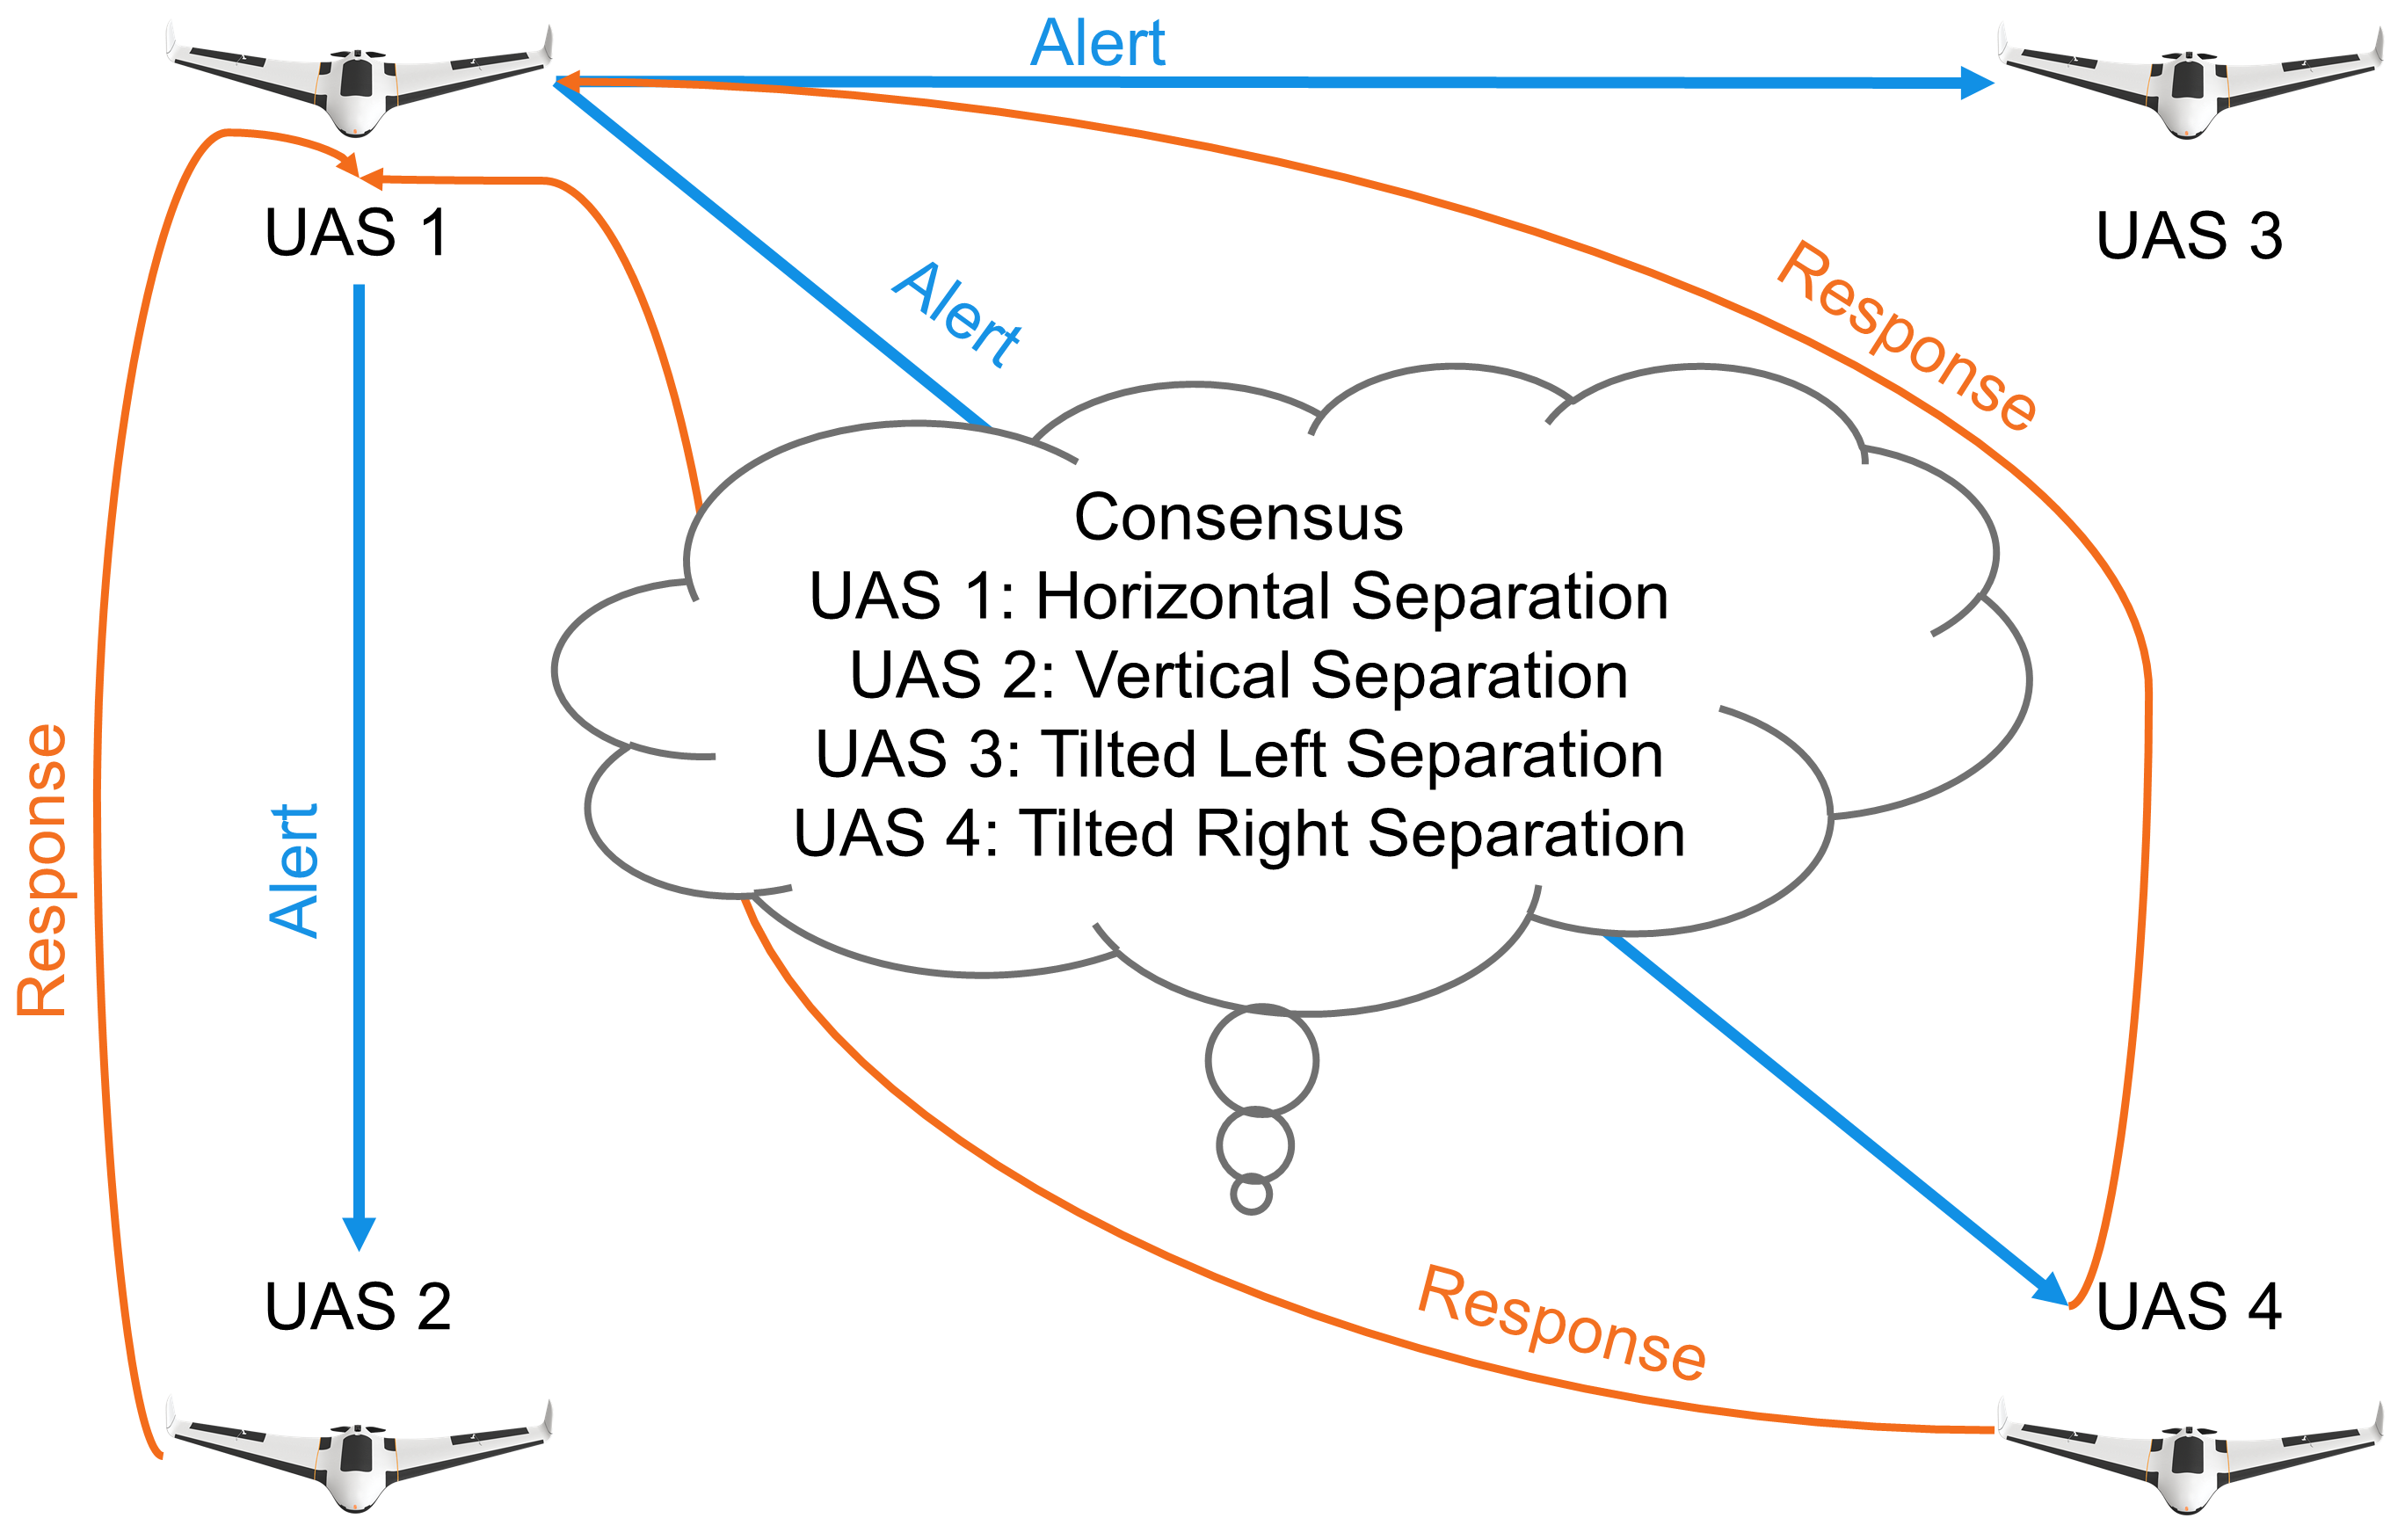
\includegraphics[width=0.7\linewidth]{\FIGDIR/RE004NonCooperativeResolution} 
    \caption{Non-cooperative conflict resolution via UAS claims.}
    \label{fig:NonCooperativeConflictResolutionUTM}
\end{figure}

\paragraph{Response mode scenario example:} The \emph{main UAS(1)} is going to collide with other \emph{UAS}(2-4):
\begin{enumerate}
    \item $UAS(1) \to UAS(2-4)$ sends position and heading notification.
    \item $\circlearrowright UAS(2-4)$ calculates possible collisions.
    \item $UAS(2-4) \to UAS(1)$ sends a response to the \emph{main UAS(1)} with claimed separation mode. 
    \item $\circlearrowright UAS(1)$ acknowledges proposed \emph{separation modes}.
    \item $\circlearrowright UAS(1-4)$ avoids each other using claimed separation mode because every \emph{UAS} achieved \emph{consensus}.
\end{enumerate}

\begin{note}
	The mutual consensus is not usually achieved via C2 communication. The most common case is \emph{assuming separation mode}. This case is shown in (sec. \ref{s:testEmergencyMixed})
\end{note}
		
%% This adds a line for the Bibliography in the Table of Contents.
%\addcontentsline{toc}{chapter}{Bibliography}
%% *** Set the bibliography style. ***
%% (change according to your preference/requirements)
%\bibliographystyle{plain}
%% *** Set the bibliography file. ***
%% ("thesis.bib" by default; change as needed)
\bibliography{thesis}

%% *** NOTE ***
%% If you don't use bibliography files, comment out the previous line
%% and use \begin{thebibliography}...\end{thebibliography}.  (In that
%% case, you should probably put the bibliography in a separate file and
%% `\include' or `\input' it here).

\end{document}
